
\section{L'écoute}


\paragraph{Ecouter ou entendre : une différence}

La définition du verbe ``entendre'' et du verbe ``écouter'' 
\autocite[pp. 361--385]{hachette:dictionnaire} nous paraît opportune
en raison de la confusion courante des deux termes :
\begin{description}
\item[Entendre] c'est  percevoir des sons, saisir par l'ouïe.
\item[Ecouter] a trois sens: 
\begin{enumerate}
	\item prêter l'oreille à; s'appliquer à entendre;
	\item prêter attention à l'avis de quelqu'un, suivre un avis;
	\item \emph{fig} suivre une impulsion,	une inspiration.
\end{enumerate}
\end{description}

\emph{Entendre} est une attitude passive par rapport au monde sonore
qui nous entoure. Nous recevons les sons sans les interpréter et cela
ne demande aucun effort. C'est une action involontaire et non
sélective.

\textit{Entendre} nous spécifie Bernard Auriol, \autocite[p. 2, ch . 1]{auriol:cle}
\begin{quote}
	<<\,suppose un son (physique), une oreille
	pour le capter, un système nerveux pour le recevoir.\,>>
\end{quote} 
Tandis qu'\textit{écouter}
\begin{quote}
	<<\,est un
	processus actif supposant préférences et répulsions pour tel son ou
	telle séquence sonore.\,>>
\end{quote}


Entendre et écouter sont donc  «\,deux
fonctions essentiellement distinctes bien qu'évoluant apparemment sur
des terrains identiques\,>>
% ancien texte {\textbf{site internet: http: auriol.free.fr} Extrait de l'entretien réalisé par
%	Bernard Auriol avec Alfred Tomatis, 1973.}.
[\dots] avec «\,l'élément conscient, facteur essentiel sur lequel repose toute la
différence entre ces deux activités\,».\autocite[]{tomatis_oreille_1991}
\pdfmargincomment{Pages des 2 citations?}
\begin{quote}
	
	<<[\ldots] \emph{Entendre, c'est en quelque sorte subir
		un son} ou un message qui nous est adressé. \emph{Ecouter, c'est désirer appréhender ce son} ou ce message [\ldots]>>
	\autocite{tomatis:education}.	
\end{quote}



Si %
\footnote{Voir point \ref{jeSuisLaMusique:viret}, p. \pageref{jeSuisLaMusique:viret}.}
\enquote{\emph{Je suis la musique que je fais ou écoute}}\autocite{viret:b}, \textbf{écouter} implique 
une conscience pour s'actualiser dans le sujet. Elle est une opération 
qui suppose une participation active dans le choix du message
ou dans la sélection d'une voix. Elle  implique la volonté,
\pdfmargincomment[color=green]{Bien!}
permet une forme de décodage: il s'agit d'une capacité.
Dans un milieu sonore important,
 bruyant, comme un café, lorsque nous lisons attentivement, nous faisons abstraction
des bruits environnants; en soi, nous les entendons parfaitement mais nous n'y
prêtons pas attention. Nous parvenons à couper les sons parasites, à nous en abstraire pour
nous concentrer uniquement sur les plus  pertinents, en l'occurrence ici ceux de notre lecture intérieure.
 La racine du mot `écouter' a des origines sanskrites et signifie \emph{partager}; nous remarquons alors à juste titre que nous écoutons le plus souvent en face de quelqu'un dans le but de dialoguer, d'échanger. Le même phénomène se réalise avec un livre qui transmet et partage des connaissances. L'écoute permet donc la communication, sous-entend le plus souvent la présence d'un être en vis-à-vis et nécessite de la  concentration. Il faut cette volonté inclue dans celle-ci  pour comprendre et rentrer en contact avec la voix de  l'écrivain qui chante dans le texte avec celle, intérieure, du lecteur.
 
 
 \textbf{Ecouter} se base certes sur une stimulation prenant sa source à 
l'extérieur mais \textbf{devant être intérieurement et  intentionnellement
	recherchée}.




Nous pouvons aussi différencier les différents types d'écoute. D'après Edith Lecourt \autocite[ch. 10 <<\,De l'écoute verbale à l'écoute musicale\,>>, p. 182.]{lecourt:decouvrir}
 on en distingue plusieurs : l'écoute verbale, musicale, plurivocale et multiple.
 L'analyse musicale qui permet la différenciation d'une voix d'un ensemble polyphonique est appelée \emph{plurivocale}. Celle qui est multiple n'est pas analytique  mais 
 \begin{quote}
 	 [\ldots] \textit{ouvre une disponibilité, met en suspens les grilles verbale et musicale} [\ldots] \emph{pour parcourir le vécu sonoro-affectif}\autocite[p. 183]{lecourt:decouvrir}.
 \end{quote}
 Employée en musicothérapie, Edith Lecourt la nomme la technique de la  \emph{communication sonore} qui peut apporter 
 <<\,des ouvertures sur l'analyse des niveaux plus archaïques de l'organisation mentale.\,>>\autocite[p. 154]{lecourt:decouvrir}	
 Par l'expérience musicale en groupe, il peut y avoir un moment particulier, de ``grâce"  nommé ``le concept d'illusion groupale", l'illusion d'une unité absolue, comme un seul corps\autocite{anzieu:groupal} dont parle Didier Anzieu.


 
Puisque \emph{écouter} implique la notion de \emph{son} et d'\emph{oreille}, nous allons dans un premier temps approfondir  la définition du son et ses caractéristiques physiques puis dans un deuxième temps aborder l'anatomie de l'oreille.

\section{Le son}
Lors d'un concert, si nous pouvions visualiser les sons qui
s'échappent de l'orchestre, ce serait un chatoiement de cercles qui se
répandraient tout autour de nous, comme 
la propagation des
ronds dans l'eau suite à un ébranlement de sa surface.
Les molécules d'air en contact avec la source sonore se déplacent et
créent une vibration.


Pour définir le son, nous avons différents paramètres,
physiologiques et psychologiques.
Il peut être
défini très précisément par un ensemble d'unités physiques chiffrées
: les décibels  et les hertz. 


\paragraph{Unités de mesures}

Un décibel\autocite[In Wikipedia]{noauthor_decibel_2018} (\SI{}{\decibel} ) est l'unité de mesure de l'intensité du son.
 Un décibel est égal à $1/10$ de bel (\SI{}{\bel}):
	$$\SI{1}{\decibel} = \SI{1/10}{\bel} $$
	 Une augmentation de l'intensité égale à \SI{1}{\bel}
équivaut à peu près à un doublement de l'intensité sonore.
		
Un hertz (\si{\hertz}) est une unité de fréquence\footnote{La fréquence est le nombre de vibrations par unité de temps dans un
		phénomène périodique.}. Équivalent à $\SI{1}{\second - 1} $. Fréquence d'un phénomène périodique
	dont la période est une seconde. \pdfmargincomment{Je laisserais tomber les multiples etc.} Ses multiples sont, entre autres,
	le kilohertz (\si{\kilo\hertz}), le mégahertz (\si{\mega\hertz}) et le gigahertz (\si{\giga\hertz}). Cette
	unité vient du savant allemand Heinrich Hertz, pionnier de la radioélectricité.

\subsection{Deux façons de définir le son et l'écoute}



De manière objective:
C'est le phénomène phy\-si\-que
d'origine mécanique consistant en une variation de pression (très
faible), de vitesse vibratoire ou de densité du fluide, qui se propage
en modifiant progressivement l'état de chaque élément du milieu considéré,
donnant ainsi naissance à une onde acoustique.

De manière subjective:	
	Il s'agit de la sensation procurée
	par cette onde, qui est reçue par l'oreille, puis transmise au cerveau
	et déchiffrée par celui-ci.\footnote{www.futura-sciences.com \pdfmargincomment{Page stp?}} 
	\index{http://www.futura-sciences.com/sante/dossiers/medecine-bruit-effets-sante-259/page/3}

Il faut aussi tenir compte de  l'impression de force sonore : la sensibilité de l'oreille
est une variable de la fréquence. Il faut 1000 fois moins de pression
acoustique pour avoir une sensation auditive à \SI{4000}{\hertz} qu'à \SI{50}{\hertz}.
Notre oreille n'a donc pas la même sensibilité pour toutes
les fréquences audibles. Il en est de même pour la sensation auditive
des basses fréquences et pour la dynamique. 

\paragraph{Ecoute objective ou subjective?}

Nous avons tous,
selon les manuels d'anatomie, la même
oreille, du moins nous pouvons reconnaître une analogie de structure. Nous devrions donc entendre et écouter la même chose
lors d'une même information diffusée tout comme le fait un enregistreur avec un micro. Pourtant il n'y a pas d'écoute \emph{passive}. Chacun n'entend pas de la même manière les mêmes
informations, chacun trie et fait son propre choix selon la fonction
d'écoute élaborée depuis l'enfance. Cette fonction sélectionne très
rapidement les mots pour être intelligible, pour se faire comprendre. En somme, tout un chacun entend ce qu'il veut bien
entendre, selon sa propre psyché.


"L'oreille a un psychisme" nous affirme Alfred Tomatis.
Nous transformons notre écoute selon nos attentes. Relevons cet 
article d'une 
étude franco-américaine scientifique
\autocite{fritz_stradivarius} au sujet des célèbres violons
Stradivarius: faite avec un protocole 
d'écoutes en aveugle avec
des violonistes professionnels et en parallèle avec un public (caché
derrière un rideau), cette étude démontre que le mythe de la suprématie
de ces instruments extrêmement chers est tombé au profit d'instruments
neufs. Nous constatons donc que le cerveau 
transforme les informations reçues selon nos attentes et qu'il joue un
rôle majeur dans notre perception.

\autocite{lemonde.fr:stradivarius}.
% 
%\footnote{\href{http://www.lemonde.fr/culture/article/2014/04/10/le-stradivarius-detrone-par-les-violons-modernes\_4398681\_3246.html}{LeMonde.fr}.}.
\autocite[p. 43]{roque:lecoute}


En est-il de même lorsqu'il s'agit de patients souffrant de dépression
ou de burnout? Sont-ce justement les souffrances dues à des situations
insupportables qui
ordonnent à notre cerveau de se protéger en obscurcissant la
perception sonore?  Ne plus écouter certains
sons permettrait-il en quelque sorte de s'échapper de la souffrance et de faire une
pause dans la douleur? Nous avons le droit et c'est un réflexe de
survie que de ne plus vouloir voir une scène affreuse et de détourner
notre regard. Nous pouvons supposer qu'il en est de même pour l'oreille ne voulant plus capter
certains sons.


 \emph{Vouloir voir, c'est viser.}  Vouloir entendre dans le but d'écouter est comparable  à
la visée de l'\oe il lorsque l'on veut collecter une
information. L'\oe il regarde avec la rétine et  vise, sous l'ordre du
cerveau, avec la macula. Dans la même idée, par l'écoute, nous avons
l'oreille et la cochlée (partie interne de l'oreille) qui permet
l'analyse des sons.

En conclusion:


 \textbf{ L'audition est la capacité perceptive du système auditif et l'écoute, c'est ce qu'on en fait.}


\section{La perception des sons et l'existence de troubles
  émotionnels}


Notre cerveau  dans sa grande complexité joue ainsi un rôle extrêmement important.
Les recherches scientifiques sont très abondantes à ce sujet et les publications n'en finissent pas de paraître.
On reconnait qu'il y a un aspect paradoxal de la musique : sa structure n'a pas une 
fonction biologique précise, nous fait remarquer Emmanuel Bigand,  chercheur, professeur 
de psychologie cognitive à l'Université 
de Bourgogne; par contre, elle peut nous faire réagir très fort, autant que la nourriture ou la 
drogue. \autocite[Voir ch. 3 p. 35, "Vous avez l'oreille musicale"]{bigand:cerveau}
D'après Isabelle Peretz
\autocite[<<\,Les agnosies auditives\,>>, pp. 205--216]{seron.baron.ea:neuropsychologie}
ainsi que le chercheur français, Hervé Platel,% 
\autocite[pp. 223--224]{platel_neuropsychology_2002}
 \enquote{le cerveau traite distinctement les aspects perceptifs et émotionnels de la 
 musique}.

Descartes nous avait inculqué trois siècles auparavant le "Je pense donc je suis". Celui-ci  a 
été bouleversé par Antonio Damasio \footnote {{L'erreur de Descartes}, Antonio Damasio, 
Ed.Odile Jacobs, 1997} 
avec sa découverte de l'intelligence émotionnelle, qui est indispensable au fonctionnement 
du 
cerveau, car  l'intelligence cognitive ne suffit pas%
\footnote{"Notre cerveau n'a pas fini de nous étonner", Entretien avec Jean-Michel 
     Oughourlian, pp. 118--119, Ed. Albin Michel, Le Livre de Poche 2012.}
Et nous avons  également le troisième cerveau, le mimétique avec les neurones miroirs que Giacomo Rizzolatti avait découvert en 1990.
 
La découverte de cette intelligence  émotionnelle est donc essentielle  pour la 
musicothérapie puisqu'on reconnaît implicitement le rôle important de la musique sur 
l'émotion.   
Ainsi le lien entre la difficulté à percevoir certains sons 
et l'existence 
de troubles émotionnels a été démontré. En d'autres termes, il y
aurait un type de vase communiquant très clair entre la perte de reconnaissance de sons et
un état dépressif.

L'étude menée par des chercheurs du CNRS, étude faite
sur des personnes déprimées avec des troubles de stress post-traumatique, atteste du 
fait qu'il y ait une diminution des seuils auditifs dans ce type de
population.
\footnote{``Les seuils auditifs des sons purs 
	sont diminués chez les personnes déprimées avec des
	troubles de stress post-traumatique.'', <<\,Pure-tone auditory 
	thresholds are decreased in depressed people with post-traumatic stress 
disorder\,>>, Journal of Affective disorders. Recherche du CNRS en collaboration
	avec Tomatis Developpement S.A. Auteurs : Stéphanie 
	Aubert-Khalfa; Emmanuelle Reynaud; Myriam El Khoury;
	Olivier Blin - INCM, UMR CNRS 6193, Jean-Pierre Granier -
	TOMATIS DEVELOPPEMENT S.A. Eva-Maria Grosse; Jean-Claude 
	Samuelian - Pôle Psychiatrie Centre, La Conception Hospital.}.

 
\begin{figure}
	\centering
	\includegraphics[width=0.7\linewidth]{images/courbesdeepressif.jpg}
	\caption{Courbes dépressif}
	\label{fig:courbes du dépressif}
      \end{figure}


Considérons ce schéma classique qui illustre la
chute des fréquences dans des zones de fréquences élevées sur un sujet
dépressif.
En ce qui concerne le Burnout,  peu d'études ont été  faites en musicothérapie
sur ce sujet, nous spécifie Felicitas Sigrist, médecin
psychiatre, psychologue et musicothérapeute à la Privatklinik
d''Hohewegg, Zürich.\footnote{Felicitas Sigrist,  
\textit{Burnout und 
		Musiktherapie}, Grundlagen, Forschungstand und Praxeologie, pp.55--90, Ed. 
	zeitpunkt musik, Reichert Verlag Wiesbaden 2016}. Par son étude, on retrouve ce 
	même lien entre son et 
émotion où elle qualifie le Burnout comme un problème de résonance "Resonanzstörung". La 
musicothérapie, qui est en plus multimodale, joue donc un rôle significatif grâce à la 
connection 
neuronale directe du système auditif avec le système limbique, d'où une activation 
émotionnelle et une  réanimation de  la capacité de résonance, dénommée comme 
étant la 
"résonance interpersonnelle"\footnote{"interpersonnelle Resonanz"F.Siegrist}.

\paragraph{L'outil "voix" en musicothérapie}

La voix en musicothérapie se révèle être un outil pertinent et délicat
à utiliser. Touchant 
directement 
l'émotion--provoquant un mouvement intérieur--la voix permet d'
éveiller l'affect
et provoque une forte stimulation. Elle n'est amenée que rarement
spontanément par le patient lui-même lors des séances et le thérapeute doit la suggérer
finement.

Selon Jacques Bonhomme, \footnote{J.Bonhomme, musicothérapeute, formateur 
  	en expression vocale, musicien, auteur de ``La voix énergie,
        instrument de nos émotions''Ed.Dangles, 1999} ``La voix est la
      résultante de la pensée résonnante et raisonnante''.
      Il nous livre ses 11 clés phonatoires pour refaire circuler dans
      le corps 
      l'émotion par l'expression de la voix qui est révélatrice des bloquages.

De nombreux tests avec 
la voix
 ont été faits pour tenter de déterminer un état dépressif 
(Test et échelle d'Hamilton). Les chercheurs de l'université de Maryland en 
2004,
en émettant l'hypothèse de la modification de l'articulation vocale 
lors d'état dépressif (on sait que la dépression provoque des changements  
neuro-physiologiques) ont révélé lors du 168\ieme\ Congrès de la Société
américaine d'acoustique, que les caractéristiques 
vocales se trouvaient modifiées lors de sentiments 
dépressifs\autocite{le_service_metronews}.

%\footnote{https://www.lci.fr/sante/et-si-on-diagnostiquait-la-depression-avec-u
%n-test-vocal-sur-smartphone-1562728.html.}.


Un test d'écoute réalisé sur un sujet dépressif nous donne également des indications
très précises sur son état
pathologique et sur la façon dont sa voix est utilisée. Jean-Pierre
Granier, psychologue, formateur et consultant Tomatis à Paris et
co-auteur de l'étude citée plus haut sur les seuils auditifs des dépressifs, nous dit qu' 
``il existe une 
interaction
constante entre le traitement auditif \textbf{et} moteur de la
voix, entre l'information sensorielle \textbf{et} les programmes moteurs impliqués
dans la parole ou le chant.'' Le programme moteur qui a été déclenché
pour la parole permet au cerveau de faire des hypothèses constantes
sur les conséquences acoustiques du geste vocal qui est sur le point
d'être réalisé. Ensuite, l'hypothèse est comparée à l'information
auditive reçue; et c'est principalement à travers l'activation de cette boucle, la
boucle audio-vocale, que peu à peu, le cerveau va modifier l'hypothèse
qu'il a construite à propos des conséquences acoustiques du geste vocal.





Et lorsque la capacité de l'écoute devient excessive et incontrôlable par le cerveau, nous 
parlerons d'autisme. Quoique
  ce domaine de recherche  soit encore en pleine investigation, il semblerait que la capacité 
  d'entendre des patients autistes soit excessive, qu'il s'agit d'une hypersensibilité aux sons 
  devenant douloureuse quand  le flux des informations est trop important et que le tri ne 
  peut pas se faire. Le cerveau entend mais ne veut pas ou ne peut plus  écouter, pour en 
  réalité, se protéger.
Selon Brigitte Harisson,  
 les dernières recherches sur le TSA (trouble du spectre autistique) affirmeraient que leur
  cerveau soit différemment connecté et qu'il ne s'agit pas d'une déficience intellectuelle ni
   d'une maladie mais d'un trouble neuro-développemental, un trouble
  d'intégration sensorielle.\autocite[Cet ouvrage propose une description unique du TSA
   (trouble du spectre de l'autisme pp. 22--23)]{harrisson.st-charles:lautisme}

Nous constatons ce lien puissant et indissociable  entre l'ouïe donnée
par l'oreille pour entendre et écouter et le cerveau exécutant ce
travail entre la 
parole et l'oreille, ce lien qui nous amène à la définition plus précise de
l'oreille: 





\section {L'oreille}


\begin{quotation}
	\char`\"{}\textbf{C'est le son qui a fabriqué l'oreille et si tu veux connaître
		le son, apprends d'abord à étudier l\textquoteright oreille\char`\"{}.}
	Hermès Trimégiste 
\end{quotation}

\subsection{L'anatomie de l'oreille}
\begin{figure}
	\centering
	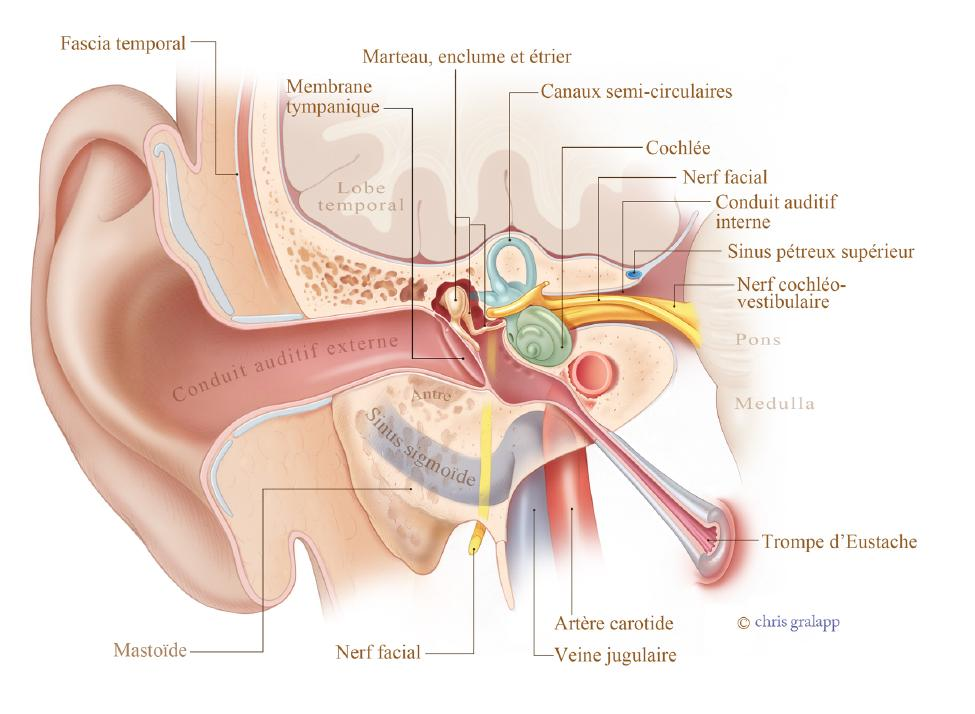
\includegraphics[width=1\linewidth]{images/20160624Berufsfeldgruppen.jpg}
	\caption[Anatomie oreille]{Anatomie de l'oreille}
	\label{fig:-20160624berufsfeldgruppen}
\end{figure}

L'oreille\autocite[ch. 8 pp. 319--321]{marieb:biologie} 
se situe à l'intérieur de l'un des os du crâne, le temporal, et plus précisément la pyramide pétreuse ou rocher. Elle se compose de trois parties : externe, moyenne, interne.

\subsubsection{L'oreille externe}

L'oreille externe\autocite[ch. 8, pp. 319--321.]{marieb:biologie}
est formée du pavillon et du méat acoustique externe
	(canal auditif). Les ondes sonores entrent dans le méat et percutent
	une membrane de \SI{60}{\milli\metre\squared}, appelée tympan, et la font vibrer. 
	Cette membrane
	sépare l'oreille externe de l'oreille moyenne. 
	Selon Alfred Tomatis,
	% au chapitre 3.3/ 4, 
	elle joue un rôle de filtre des graves et d'amplificateur des aigus.




\subsubsection{L'oreille moyenne}

L'oreille moyenne se trouve dans l'os temporal constituée de petites
cavités dont une, centrale, qui est la caisse du tympan. Sa limite
médiale est une paroi osseuse percée de deux orifices, la fenêtre
du vestibule et la fenêtre de la cochlée. La trompe auditive ou d'Eustache
est un conduit oblique qui relie l'oreille moyenne à la gorge et sert
à équilibrer la pression de l'air entre l'oreille moyenne et l'extérieur.
Les trois osselets de l'ouïe sont : le marteau, l'enclume et l'étrier
(les plus petits os du corps). Ils transmettent les vibrations du
tympan aux liquides de l'oreille interne. Le marteau et l'étrier se
trouve dans l'os temporal constituée de petites cavités dont une,
centrale, qui est la caisse du tympan. 
% OGA: répétition ici, c'est pourquoi j'ai commenté
%Les trois osselets de l'ouïe
%sont : le marteau, l'enclume et l'étrier (les plus petits os du corps);
Le marteau et l'étrier sont commandés chacun par un muscle. D'après
Tomatis, son rôle est double : protéger l'oreille interne des sons
trop forts et celui de cibler les sons à écouter.

\subsubsection{L'oreille interne et le labyrinthe osseux}

\begin{figure}
	\centering
	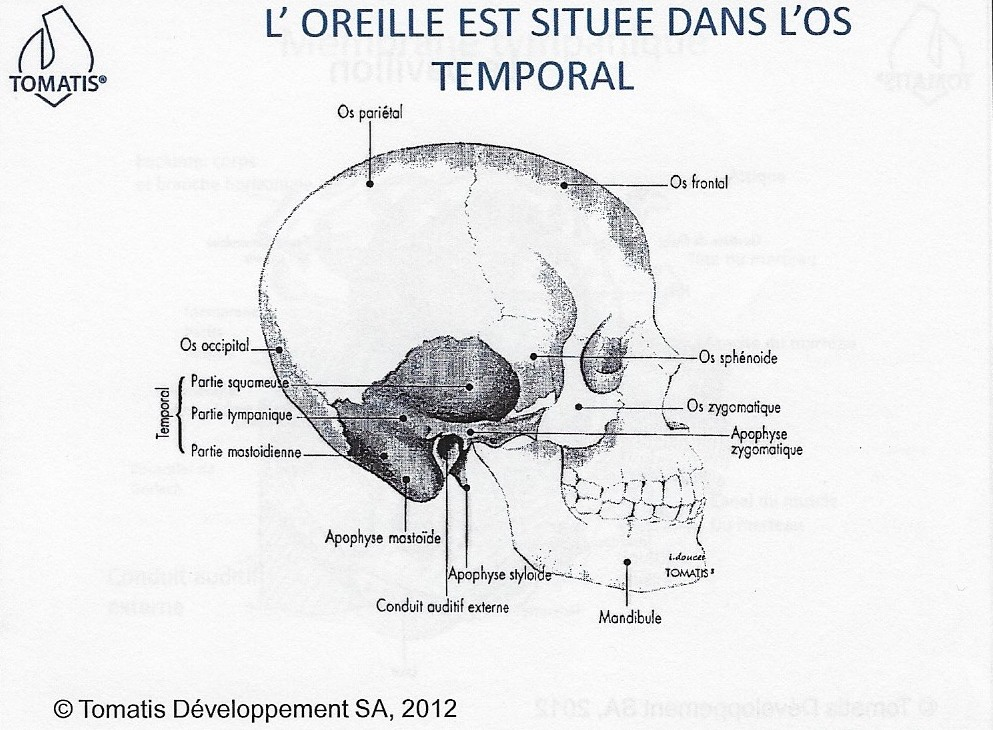
\includegraphics[width=0.7\linewidth]{images/Loreilleostemporal_crane.jpg}
	\caption[L'os temporal]{L'os temporal}
	\label{fig:loreilleostemporal18}
\end{figure}

L'oreille interne est l'organe de l'audition. Il
est constitué d'une coque osseuse d'une très grande densité (la plus
importante du corps), contenant un corps membraneux qui en épouse
la forme. 
L'oreille interne est une enfilade de cavités osseuses portant 
le nom de \emph{labyrinthe osseux}. Il comprend trois subdivisions : 
\begin{enumerate}
	\item la cochlée;
	\item le vestibule du labyrinthe;
	\item  les canaux semi-circulaires.
\end{enumerate}

Le labyrinthe
osseux est rempli de périlymphe, un liquide. Et dans ce périlymphe
flotte le labyrinthe membraneux qui contient lui-même un liquide
plus épais appelé endolymphe. Ils jouent leur rôle dans l'équilibre
statique et dynamique. Le vestibule et les canaux semi-circulaires
sont les organes de l'équilibration; la cochlée ou
limaçon est l'organe de l'audition. 

\subsubsection{Le canal auditif}
\pdfmargincomment[color=yellow]{répétition avec oreille externe}
Les ondes sonores entrent dans le méat et percutent
une membrane de \SI{60}{\milli\metre\squared} appelée \emph{tympan}, et la font vibrer. Cette membrane
sépare l'oreille externe de l'oreille moyenne. Selon Tomatis, elle
joue un rôle de filtre des graves et d'amplificateur des aigus.



\subsection{La physiologie de l'audition}

Le  son crée un chemin dans 
l'oreille\autocite[chap. 8, pp. 322--324]{marieb:biologie} jusqu'au cerveau.

Chaque son parvenant à l'oreille entre dans le pavillon et se propage
dans le conduit auditif. Les vibrations de l'onde sonore mettent en
mouvement le tympan lié aux trois petits os (marteau, enclume, étrier).
Les osselets ont le rôle de transformer et d'amplifier les vibrations
aériennes et de les transmettre à l'oreille interne via la fenêtre
ovale.

Le rapport de levier effectif entre le marteau et l'enclume
(de l'ordre de 20), d'une part, et le
rapport de surfaces entre le tympan et la platine de l'étrier
(\SI{30}{\milli\metre\squared}) d\textquoteright autre part font du système tympano-ossiculaire
un véritable amplificateur permettant à l\textquoteright énergie sonore
d\textquoteright être transmise presque intégralement à l\textquoteright oreille
interne.

A partir de 80 dB, un réflexe protecteur (stapédien) est mis en place
afin de réduire la transmission des pressions vers l\textquoteright oreille
interne, par l\textquoteright intermédiaire des osselets et des muscles
qui rattachent le marteau et l\textquoteright étrier aux parois de
la caisse du tympan. Il s'agit ainsi d' un procédé mécanique qui amplifient
les vibrations atteignant la cochlée. 
\begin{quotation}
	La cochlée à son tour ``va transformer ces vibrations en impulsions
	nerveuses véhiculées par le nerf auditif.'' (\dots) Les cellules ciliées
	tapies dans la membrane cochléaire ``transforment ces vibrations
	en messages électriques, circulant dans le nerf auditif. (\dots) Et
	ces informations vont ``se diriger vers le cortex cérébral, via plusieurs
	relais. (\dots) ``Comme certaines fibres issues de chaque oreille croisent
	la ligne médiane, chaque aire auditive reçoit des signaux des deux
	oreilles.'' De plus, ``tout au long du trajet, le message subit
	des transformations dues aux caractéristiques de l'activité des neurones.''
	Retenons que `` les cellules ciliées proches de l'étrier sont activées
	par les sons aigus, et celles situées au sommet de la cochlée le sont
	par les sons de basse fréquence''. (\dots)``Une scène auditive est
	mêlée d'un ensemble d'ondes acoustiques et son analyse se ferait non
	seulement tout au long du système auditif avec des indices comme la
	fréquence et l'intensité mais aussi au-delà, pour utiliser les informations
	liées aux autres sens ou au contexte.'' \autocite[chap.1, pp.~15--16]{bigand:cerveau}
%	\footnote{\textbf{Le cerveau mélomane} Le cerveau mélomane,2011}, chap.1, pp.~15--16.}
\end{quotation}


        \begin{figure}
	\centering
	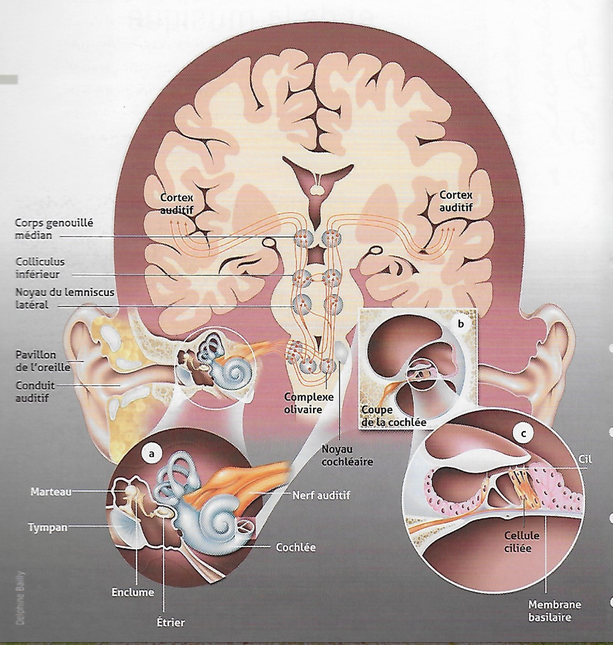
\includegraphics[width=1\linewidth]{images/schemacerveauoreillebigand.png}
	\caption[Schéma du déroulement]{La perception des sons et de
          la musique, E.Bigand, ``Le cerveau mélomane''Ed.Belin}
       
	\label{cerveauoreillebigand1}
\end{figure}




\section{Le test d'écoute et l'audiogramme}

\subsection{Qu'est-ce un test d'écoute?}

De manière générale, le test d'écoute se  définit comme étant de nature verbale, avant tout 
psychologique et mettant principalement l'accent sur la communication
et la capacité d'empathie.





\subsection{L'audiogramme}

Dans le milieu médical, on le nomme test d'audition ou audiogramme. Il
sert à mesurer les seuils d'audition des sujets, grâce à l'audiomètre. Cet 
appareil français avait été mis au point en 1933. Les Américains
ont repris ces travaux pendant la dernière guerre pour pouvoir dépister
les dommages subis par ceux qui conduisaient des avions ou d'autres
engins similaires bruyants.
  L'audiogramme est une épreuve d'ordre physiologique. Ce test peut faire partie des examens  pratiqués en otologie\footnote{otologie : branche de la médecine
  	qui étudie l'oreille et ses maladies.} pour poser un diagnostic. 
   C'est un examen à partir duquel se
  dessinent les données dénommées étiologiques\footnote{étiologie : étude des causes
  	d'une maladie} pour détecter un trouble de la fonction auditive. Un pronostic pourra définir le mode de thérapie
médicale, chirurgicale, prothétique ou rééducative. La procédure
technique inclut des paramètres et manipulations propres au corps
médical des auscultations O. R. L. et  n'est pas systhématique.

Il n'y a pas d'épreuve psychologique. 




\section{Le test d'écoute en musicothérapie}

Les musicothérapeutes ne se lassent pas d'explorer l'alliage du son
 et de la psychologie, et vice
 et versa, les psychanalystes, les psychiatres, les psychologues
 s'intéressent à intégrer le son dans leur travail. Par ce truchement,
 un travail différent est fait pour une anamnèse plus large et
 plus profonde du patient. Le son permet de donner un miroir
 psychologique de la personne par un chemin détourné. Par cette
 démarche, ils diffèrent de certains tests psychologiques usuels
 et se nomment bilans psycho-musicaux. On peut les trouver sous
 plusieurs formes: soit avec l'audition d'\oe uvres
 musical où les patients répondent à une grille précise de questions
 selon les oeuvres, soit en trois parties, avec un entretien,
 une écoute musicale (partie réceptive) et une production musicale
 (partie active).

 
 On reconnait le rôle éminemment important que peut jouer la musique
 dans les traitements psychiatriques et ce type de test devient
 fréquent dans beaucoup d' établissements. Ils le sont aussi  par principe de précaution et
 par souci d'ajuster au plus près une
 musicothérapie. Rolando Benenzon, Jacqueline Verdeau-Paillès, Edith
 Lecourt sont des musicolthérapeutes-médecins-psychiatres qui ont contribué à la mise en place de ce
 type d'évaluation.

  
\section{La musicothérapie et la psychothérapie}
\label{musicothEtpsycho}

	 La musique s'est révélée  être un important support d'expérimentation.
	 Rolando Benenzon, Jacqueline Verdeau-Paillès, Edith
         Lecourt, Helen Bonny ont su intégrer dans leur exercice professionnel l'utilisation du son comme
          élément facilitant l'exploration psychique. 
	  Ils ont élaboré des procédures de prise en charge des patients en 
	  musicothérapie en soulignant  
	   l'importance d'un tel support dans la  communication et
           l'introspection.
           D'autres comme Nevjinsky, Bernard Auriol, Jacques Bonhomme
           et Alfred Tomatis ont développé leur propre concept avec
           des voies différentes mais toujours au service de l'humain. 

\subsection{Le test d'écoute et bilan psycho-musical}
	  
\subsubsection{Rolando Benenzon}
Rolando Benenzon
	  
	  \label{benenzon}
	  Le professeur et docteur Rolando Omar Benenzon s'est inspiré et a basé sa technique 
	  musicothérapeutique à partir de 1969 
	  sur Jung.  Freud, Winnicott, Watzlawick l'ont également imprégné. 
	  Influencé par le concept de l'objet sonore  avec P.Schaeffer et C.Sachs 
	  ainsi que par les grands pédagogues musicaux comme Willems,
          Dalcroze ou Kodaly, sa définition de la musicothérapie est celle d'une musico-psychothérapie  
	  \emph{\textsl{qui utilise les expressions corporo-sonoro-non verbales.}}, 
	  centrée sur le concept d'identité sonore, l'"\textit{ISO}".

        \subsubsection{Edith Lecourt} est une Docteur ès lettres et sciences 
        humaines, psychologue clinicienne, psychanalyste et musicienne à l'Université René Descarte-- Paris 
        V),musicothérapeute, cofondatrice  et vice-présidente de
        l'Association française de musicothérapeute. Ses recherches
        actuelles portent sur la psychanalyse de groupe, les
        dimensions subjectives du sonore  et l'émotion esthétique en thérapie.
    
 	 
        R.Benenzon et E.Lecourt ont  recherché la place qu'occupe le sonore dans la vie d'un 
        patient, et on peut supposer qu'ils ont sans doute perçu l'idée générale et 
        conductrice de \emph{la méthode projective}, 
        en terme 
	    <<\,d'investigation dynamique et holistique de la
        personnalité\,>>. Les tests projectifs sont devenus à partir
        de 1939 un des instruments très utilisés en psychologie
        clinique. Ils réunissaient trois épreuves : le test
        d'association de mots de Jung (1904), le test des taches
        d'encre de Rorschach (1920) et le TAT (test d'histoires à
        inventer) de Murray (1935)\autocite[ch.~1, p.~13]{anzieu.chabert:methodes}.
		

	
\paragraph{Modèles originaux de tests musicothérapeutiques}

Inspirés par ces divers courants, Jacqueline Verdeau-Paillès, Helen Bonny et Fern Nevjinsky ont mis au point au fil de leur
pratique des modèles originaux de tests musicothérapeutiques
spécifiques. Selon Edith Lecourt,
(2017)\autocite[ch.~3, p.~84]{Les arts-thérapies,Ed.Armand-Colin}
c'est Jacqueline Verdeau-Paillès qui a conçu à
l'origine le bilan psycho-musical pour ses patients dans son service
de psychiatrie. Les recherches de R.
Benenzon ont aussi joué leur rôle \autocite{benenzon:musicotherapie}  pour l'élaboration d'un
test similaire; elles se passaient quasi en
parallèle et on peut supposer qu'ils se soient co-influencés. Sans
parler de J.Jost qui avait également commencer à construire un test dans ce sens.




\subsubsection{Jacqueline Verdeau-Paillès}

 Ainsi, la psychanalyste Jacqueline Verdeau-Paillès a 
intégré à partir de 1985 la psychanalyse avec le son. Elle a  introduit
 le sonore 
sous forme réceptive avec un test d'audition d'\oe uvres pour réaliser
une relation analytique\autocite{verdeau-pailles:bilan}.

Par l'entretien, on recherche quelle est la place qu'occupe la
musique et le sonore dans la vie d'un patient. Puis par un test
d'audition d'\oe uvres et par un test actif, on peut évaluer la
réceptivité et les possibilités de communication par ce médium. On
observe les réactions comportementales, les productions sonores et les
verbalisations. La technique du montage en U qui débute de 3 à 10
morceaux de 3 à 4 minutes, selon l'âge, le milieu, la culture, chacun
en fondus enchaînés, est aussi une technique qui amène progressivement le patient à la détente
et au verbal.
La synthèse de ces observations permet de poser une hypothèse de
travail, d'établir un projet thérapeutique, de savoir s'il y a
indication ou contrindication.





\subsubsection{Helen Bonny} 


Helen Bonny (USA) était une musicothérapeute,
musicienne et psychothérapeute, qui a mis au point dans les années 70
une technique particulière, le GIM,<<\,Guided Imagery and Music\,>>
l'imagerie guidée et de la musique. Selon GIM
Trainings\autocite{gim_site} la
musique associée à la thérapie libère par l'émotion et relie le
conscient à l'inconscient.\footnote{\textsl{The Evolution of Guided Imagery and Music}, 
	by Helen Bonny, Ed. by Lisa Summer (2002), p. 7.}
 C'est une forme réceptive de travail
en musicothérapie, avec comme principales influences Carl Rogers, Abraham Maslow et Carl Jung; 
elle  consiste en une longue anamnèse avec le
patient qui permettra de cibler le programme de musiques appropriées. 
(des \oe uvres de compositeurs tels Beethoven, Brahms, Debussy,
Mozart, Rachmaninov ou Vivaldi.)






 \subsubsection{Fern Nevjinsky et le test de Rorschach}
 
 De son côté, Fern Nevjinsky a développé à partir du  test de Rorschach un test psycho-musical avec des morceaux
de musique en association libre. Il utilise ainsi le test
musical en complémentarité de celui de Rorschach%
\autocite[Fern Nevjinsky, maître de conférences à l'Université de Rouen, musicien, psycho-analyste. 
Comparaison des modalités de projection et d'expression au test de Rorschach et à un test psycho-musical pour des adolescents de 13 à 16 ans.]{nevjinsky:adolescence}.  
Il nous dit  que  «\,[\ldots] la
portée diagnostique du test fait avec des sons purs, en se limitant à
l'identification, est insuffisante; mais, si la consigne est libre ---
dire ce que le son signifie --- toutes les perceptions erronées sont
le point de départ d'une expression fantasmatique en relation avec le
passé du sujet, ses souvenirs. [\ldots] 
Il prouve  la valeur privilégiée du son comme éveil
des affects liés à des conflits qui n'apparaissent pas dans
l'entretien ou dans les tests visuels.  [\ldots] A un niveau
psychanalytique, par le biais de la régression, elle peut amener le sujet à abandonner une partie de sa vigilance défensive.\,»\pdfmargincomment{pages?}

Nous constatons que les techniques divergent quelque peu mais restent
reliées au concept essentiel, c.à.dire: 

La musique favorise  <<\,\emph{l'expression et le développement
	de la pensée}\,>> et  va <<\, [\ldots] \emph{permettre la prise de conscience des processus pathologiques développés} [\ldots]\,>>\footnote{Source : ASSOCIATION AMARC,
  Association de musicothérapie, recherches cliniques et
  applications). \pdfmargincomment{references de l'article AMARC?}}.

Elle est un outil non-anxiogène, déclencheur des expressions et provoque
l'éveil des affects dans  leur verbalisation qui sera recueillie lors
du bilan psycho-musical.
 
  \subsubsection{Jacques Bonhomme} \footnote{J.Bonhomme, musicothérapeute, formateur 
  	en expression vocale, musicien, auteur de ``La voix énergie,
        instrument de nos émotions''Ed.Dangles, 1999}  a 
      été formé par A.Tomatis, déjà cité. Il se sert du même test d'écoute
      que lui et l'enseigne dans son ``Ecole de la voix'' lors des
      formations qu'il donne. Il a étendu cette  forme active de musicothérapie
      spécifiquement avec la voix 
     et a acquis une
      très grande expérience qu'il transmet en   
      faisant référence au lien entre l'écoute, la voix et la vie émotionnelle.

 \subsubsection{Bernard Auriol}

Bernard Auriol\footnote{Médecin psychiatre, psychothérapeute, 
	né en 1938, a écrit plusieurs ouvrages, dont : \textsl{Le son au subjectif présent}, \textsl{La clef des sons, Éléments de psychosonique}, \textsl{Méditation et
  psychothérapie}.}
a étendu ses recherches sur le son, la psychosonie, 
tout en s'inspirant également des
travaux d'Alfred Tomatis, avec lequel il s'est formé et sur lequel
nous donnerons plus de détails.

Le terme \emph{psychosonique} a été créé en 1991 par Bernard Auriol pour
désigner la discipline qui cherche à évaluer et décrire les effets du
son sur l'être vivant ainsi que les éléments
subjectifs manifestés par l'expression sonore:  la
voix. 
La psychosonique s'étend aux éléments
symboliques, psychodynamiques, inconscients et subjectifs du processus
d'écoute. En psychanalyse pour lui, ce n'est pas qu'une affaire de
texte et de parole mais il souligne l'importance de la voix porteuse non seulement
d'imaginaire, de symbolisme mais aussi ``la matérialité insaisissable
des vibrations qui empruntent ``( et là il cite )``...les voies mystérieuses de
l'affect proprement auriculaire''.(Lacan,1963)
``Ecoute ! Ecoute !
Oser Psychanalyser l'écoute
(Chapitre 13 de "La Clef des Sons")
Dr Bernard Auriol''



Sa passion pour le son l'a conduit, entr'autres, à mettre au point des tests
d'écoute, inspirés de ceux d'A. Tomatis.
       
\subsubsection{Alfred Tomatis}


A notre sens, le  test d'écoute le plus neutre, le plus objectif, révélateur de l'état d'écoute
du patient, qui permet de faire <<\,\emph{chek-up} d'entendre et d'écouter\,>>
 --qui donne des indices sur la façon dont le sujet prête l'oreille
 aux sons autour de lui et sur l'évolution de son écoute au fil des thérapies--,
celui qui regroupe l'ensemble de ces
données est en effet le test d'A.Tomatis.
Sa technique d'évaluation
de l'écoute est concrète, ce qui signifie qu'elle ne
sollicite pas un travail intellectuel au niveau du verbal.
Les réponses sont gestuelles.

Puisque notre choix s'est posé sur ce test Tomatis, nous allons
aborder plus largement cette méthode avec pour objectif de savoir
- s'il est un outil valable et utilisable en musicothérapie,
- s'il permet de déceler une possible corrélation avec l'état
psychique du patient,
-s'il amène un éclairage différent sur les tests psychologiques
utilisés en musicothérapie.
